
\chapter{Evaluation and Testing}

In this chapter, we evaluate and test the implemented history system to find out how useful it is.

First, we explain what does it mean for a system of a tool to be useful. Plus we point out the specifics of estimating the usefulness of history systems.

Second, we use a few real life scenarios to show the advantages of our search application in practice. Using these scenarios we compare different methods to search for and retrieve entries from shell history.

Third, we introduce metrics to quantitatively evaluate our history system. Then, we use the metrics to compare our search application with another state-of-the-art history tool.

Fourth, we describe how we incrementally improve the system since the initial release. The community of existing users makes it possible to get impressions, ideas, and feedback. 

Finally, we show additional use cases that are possible to fulfill using our search application. 

\section{Usefulness of history tools}

The goal of this work is to design and create a history system that is useful. 
We want people to use the tool because it both solves their workflows and it is easy and pleasant to use.

The usefulness of the system is determined by its utility and its usability.\cite{nielsen2012usability} Utility is a quality attribute of the system that assesses if the system provides the features that users need.\cite{nielsen2012usability} Usability refers to how easy and pleasant are the features to use. Any useful system needs to have both good utility and usability.

In following sections we describe what utility and usability means for history tools specifically.

\subsection{Utility}

History systems should make it cheaper, in terms of mechanical and cognitive activity, to retrieve history entries than to type them again.\cite{greenberg1993computer}

Retrieving command line entries from history saves us typing. Even small savings in typed characters make a difference because typing is an error-prone activity; A significant amount of time is usually spent detecting and fixing errors. According to \cite{whiteside1982people}, typing only accounts for about a half of all key strokes during text editing. 

%"Command line entry involves not only typing the final correct characters, but also the time it takes to detect and correct typing errors. Actual character savings are likely double the theoretical ones" \cite{whiteside1982people}

Before typing the command line entry, the user has to think of what to type. In many cases, this might be more difficult than the act of typing out the command line entry.   

%Generally, recognizing and selecting and activity is considered easier than recalling it or regenerating it. \cite{greenberg1993computer}

To evaluate the utility of our history system we use metrics that are based on how many characters users retrieve from history and how much information is required for a successful retrieval.

\subsection{Usability}

Usability can be broken down to five following quality components.\cite{nielsen2012usability}

\begin{itemize}
    \item Learnability
    \item Efficiency
    \item Memorability
    \item Errors
    \item Satisfaction
\end{itemize}

Learnability assesses how easily can users complete basic task when they use the system for the first time. For example, non-standard key bindings that are not shown on the screen could make the interface difficult to use.

Efficiency means how quickly can users achieve their goals once they already know how to use the system. If the design requires users to complete too many steps to accomplish their goal it will slow them down. 

Memorability represents if the users can proficiently use the system after they did not use it for a while. 

We also want to know how many errors people make while using the system. Does the design make it easy to recover from errors? For instance, if there would be no way to revert ones actions the users might learn to use the system slowly and carefully. 

Satisfaction assesses if it is pleasant to use the system. For example, system that unpredictably fails will likely cause its users to distrust it. Users might not enjoy to use a system they do not find reliable. 

%Learnability: How easy is it for users to accomplish basic tasks the first time they encounter the design?
%Efficiency: Once users have learned the design, how quickly can they perform tasks?
%Memorability: When users return to the design after a period of not using it, how easily can they reestablish proficiency?
%Errors: How many errors do users make, how severe are these errors, and how easily can they recover from the errors?
%Satisfaction: How pleasant is it to use the design?

\subsection{Issues with testing history tools}

Ideally, we would want to perform usability testing with users; This would help us to find usability issues of the system and estimate its overall usability.

When conducting usability testing we want to see users perform real tasks using the system. It is necessary to prepare testing scenarios for users to follow during the testing session.

However, history tools cannot be tested as easily as other applications or websites.
Unlike with other applications, scenarios for our history search application are heavily dependent on the personal workflows of the specific user and his history.


We would need to prepare personalised scenarios for individual users based on their shell history and their usage of the history mechanisms.
This is possible but it proved to be too time consuming for us to use in this work.

We released this project a while ago and we iteratively improve it. Because of that we got a lot of feedback and many chances interview our users. We also collected some shell history and usage data from our users. We use this data to demonstrate the usefulness of our solution.

\section{Evaluating real life scenarios}

In this section, we compare our history searching with other history tools based real life scenarios. We have collected shell history with usage from some of our users and chose specific situations to showcase the advantages of using our history search application.

We found situations when people have used either Hstr\cite{toolshstr} or our search application to retrieve history entries. We took the shell history available at the time and fed it into three different history tools. The tools we test are standard reverse search, Hstr, and our search application. Now, we compare how difficult it is to retrieve the desired history entry using these three history tools.


\subsection{First scenario}

In the first real life scenario, the user is trying to retrieve following history entry: 

\begin{verbatim}
ansible-galaxy install -r requirements.yml -p roles
\end{verbatim}

%\verb|/Users/vit.listik/git/szn/laas/ansible-etcd|

\paragraph{Reverse search}
If the user used reverse search and typed \verb|ansible| as a query, the desired history entry would be twenty results away. As we described earlier in section  \ref{workflow-search-w-implicit-context}, pressing \verb|CTRL-R| twenty times while reading the results one by one is quite inefficient.

Instead of using \verb|ansible| as a query and going through many results, the user could use a more specific query. Using \verb|ansible-g| as a query returns the desired history entry as the first result. In this case, however, the user has to remember more information about the history entry.

\paragraph{Hstr}
Now, we look at how the user could use Hstr to retrieve the same history entry.

Typing \verb|ansible| returns the history entry on twentieth position on the page. Unlike with the reverse search, the user could fairly quickly scan the page and select the desired history. 

However, it could be faster to extend the query to further filter the results. Unlike with the reverse search, the user can use any part of the command line entry as a query because Hstr breaks the query down to separate words. Extending the query to \verb|ansible ins| returns the desired entry as the first result.

% Hstr requires less knowledge and less typing than reverse search. Plus selecting a twentieth result in Hstr is realistic unlike in reverese search.

\paragraph{Our contextual search application}
Finally, we compare how our search application performs compared to the other two options.

After the user opens the search application the desired result is already in the third position. The user does not even have to specify a query because the search application returned the history entry based on the current context.

Typing \verb|ans| as a query brings the desired history entry to the first position. As we can see, our solution requires less knowledge and less typing to retrieve the desired history entry than both Hstr and reverse search. 

\subsection{Second scenario}

In this second scenario, the user wants to retrieve the following history entry.

\begin{verbatim}
ansible-playbook infra_os_deploy.yml -i inventory_example.ini -b
    -u debian -D
\end{verbatim}

%\verb|~/git/szn/laas/ansible-playbooks|

\paragraph{Reverse search} 
First, we look at how the user could use the reverse search to retrieve the desired history entry.

Using \verb|ansible-playbook| as a query returns the history entry as thirty-first result. This is practically unusable. Plus this query is very hard to extend.

The user could chose to delete the query and use a different one. Coming up with a usable query is hard in this case; For example, typing \verb|inventory| or \verb|debian| returns the history entry as second and third result respectively. In contrast, using \verb|infra| or \verb|deploy| leaves the entry well beyond the reach of the user. 

\paragraph{Hstr}
Second, we describe how Hstr can be used to retrieve the previously mentioned history entry.

Typing \verb|ansible| does not return the desired history entry. However, the user can quite easily extend the query to \verb|ansible inf| which returns the history entry as a first result. 

We can see how the ability use multi-word queries makes it much easier to use Hstr than reverse search.

\paragraph{Our contextual search application}

Third, we compare our search application with both previous methods. 

When the user launches the application, he can already see the desired history entry as the eight result on the page. This is possible because the current context matches the context of the desired history entry. 

As before, typing \verb|ans| as a query brings the desired history entry to the very first position on the page. 

In situations like this one, our search application makes it very easy to retrieve the desired history entry. Hstr provides an reasonable to retrieve the entry but using context gives advantage to our solution. Reverse search is nearly impossible to use in this scenario.



\section{Metrics}

In previous section, we demonstrated the advantages of using the contextual search application using specific situations. We saw how reverse search can be very ineffective. In contrast both Hstr and our search application performed adequately.

Here, we introduce metrics we will use to evaluate the utility of the search application. We will later use the metrics to compare Hstr with our search application. 

\subsection{Number of saved characters}

The first metric is the number of saved characters. It represents the typing saved by the user.

Since we compare two similar history tools we assume that the number of key strokes needed to select a history entry is similar once the entry appears on the screen. Because of that we are not subtracting the key strokes needed for selection inside the history search applications.

\subsection{Amount of required knowledge}

The second metric represents the amount of knowledge the user needs to retrieve the history entry. We measure the amount of required knowledge in the unit of "knowledge tokens".

Knowledge tokens are substrings of the command line entry that consist of alphanumerical characters and are at least four characters long. We chose this definition of a knowledge token because it matches the type of information people usually remember and use for searching. We observed this behavior in our users. 

For example, imagine that you are searching for the following history entry.

\begin{verbatim}
curl -O -L https://api.github.com/repos/curusarn/resh/releases  
\end{verbatim}

You would probably use something like \verb|curl github| as a query. The longer chunks of letters represent meaningful information while symbols are repetitive noise.



%\redtext{...........}
%When applying this metric we want it to be deterministic. This means that we need an automatic way to turn a command line entry into tokens 


\section{Applying metrics}

In this section, we apply the previously introduced metrics. We use the metrics to compare Hstr with our search application.

\subsection{Collected data}

We have collected shell history and usage data from a few of our users. Out of these users there is a single user that was previously using Hstr and switched to our history search application. We use the data from this user to compare the utility of these two history applications.

During five months of collecting the data, this user has successfully used Hstr 121 times and our history search application 69 times. For each of these data points we know what command line entry the user executed. 

We also know when the event happened. This means that we can take the shell history that was available at the time and feed it into Hstr and our search application. This way we can see what results would these history tools return at that time. We can compare how difficult would it be to retrieve the desired history entry in either of the history tools. 

\subsection{Simulating history searching}

To evaluate the history tools we simulate searching and use previously introduced metrics compare them.

First, we look at the results that are returned without any query. If we can find the desired history entry in the first twenty results then we are done. We use the first twenty returned results because it is an amount that fits into small terminals. 

When we do not find the result, we add a single word to the query and we search again. We keep adding more words to the query until we find the desired history entry. 

After we find the desired result we know how the search tool performed; We know how many characters were retrieved from history and we also know how many words we needed to use as a query.

\subsection{Comparing Hstr with our search application}




\begin{itemize}
    \item We want to compare these tools
    \item We have usage from the same user from time when they used Hstr and when they used our solution
    \item People use different tools differently; We saw a difference in usage of Hstr and in the usage our search application. It seems that users adapt to whatever tool they have available.
    \item Because of this we take the usage from both of these tools separately. And then for each "usage" we simulate how well would both of the history tools perform.
\end{itemize}




Figure \ref{eval-metrics-plot-cmds-hstr} comparing hstr and our search application in situations when the user originally used Hstr

Figure \ref{eval-metrics-plot-cmds-resh} comparing hstr and our search application in situations when the user originally used our search application

\begin{itemize}
    \item We can see that our application requires more knowledge than Hstr in figure \ref{eval-metrics-plot-cmds-hstr} which is expected because user origianally used Hstr for this history searching
    \item In figure \ref{eval-metrics-plot-cmds-resh}, we see the opposite. Our shearch application requires less knowledge than Hstr because user originally used our search application for these history searches.
\end{itemize}


Figure \ref{eval-metrics-plot-chars-hstr} comparing hstr and our search application in situations when the user originally used Hstr


Figure \ref{eval-metrics-plot-chars-resh} comparing hstr and our search application in situations when the user originally used our search application

\begin{itemize}
    \item Figures \ref{eval-metrics-plot-chars-hstr} and \ref{eval-metrics-plot-chars-resh} show something similar but here we use the number of saved characters (normalized per number of retrieved history entries). 
    \item Here, we can see that Hstr is on average more successful at finding shorter history entries when applied to the usage data from our search application.
    \item This is not surprising; It matches findings from previous research\cite{greenberg1993computer} where directory sensitive history returned longer history entries because. More specific history entries generally tend to be longer and generic and common command line entries tend to be shorter.
\end{itemize}

We conclude that our history search application performs on par with Hstr. Using contextual search as a default is a reasonable trade off.

One important thing we should point out is that we have used the same full shell history for both Hstr and our search application. Hstr normally only uses standard shell history which might be missing some history entries. 

In all previous comparisons we give the benefit of the doubt to Hstr. 

\clearpage
\begin{figure}[h!]
\centering
\tmpframe{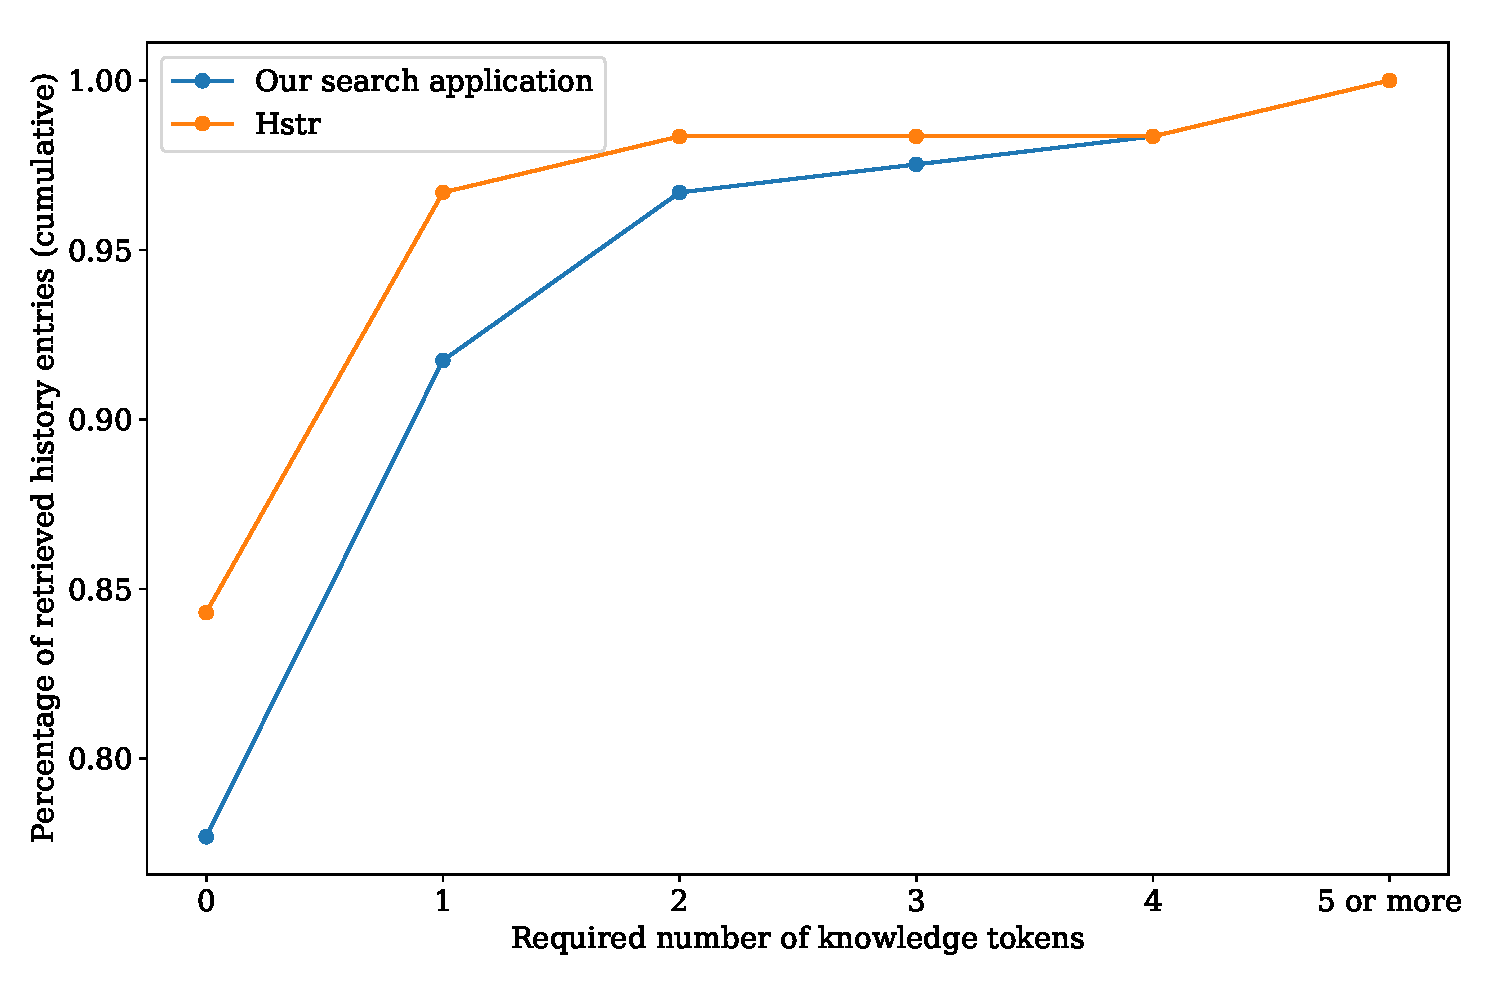
\includegraphics[width=0.97\linewidth]{figures/testing/testing-metrics-cmds-hstr.pdf}}
\caption{Cumulative percentage of retrieved history entries as a function of required knowledge (Invocations of Hstr)}
\label{eval-metrics-plot-cmds-hstr}
\end{figure}

\begin{figure}[h!]
\centering
\tmpframe{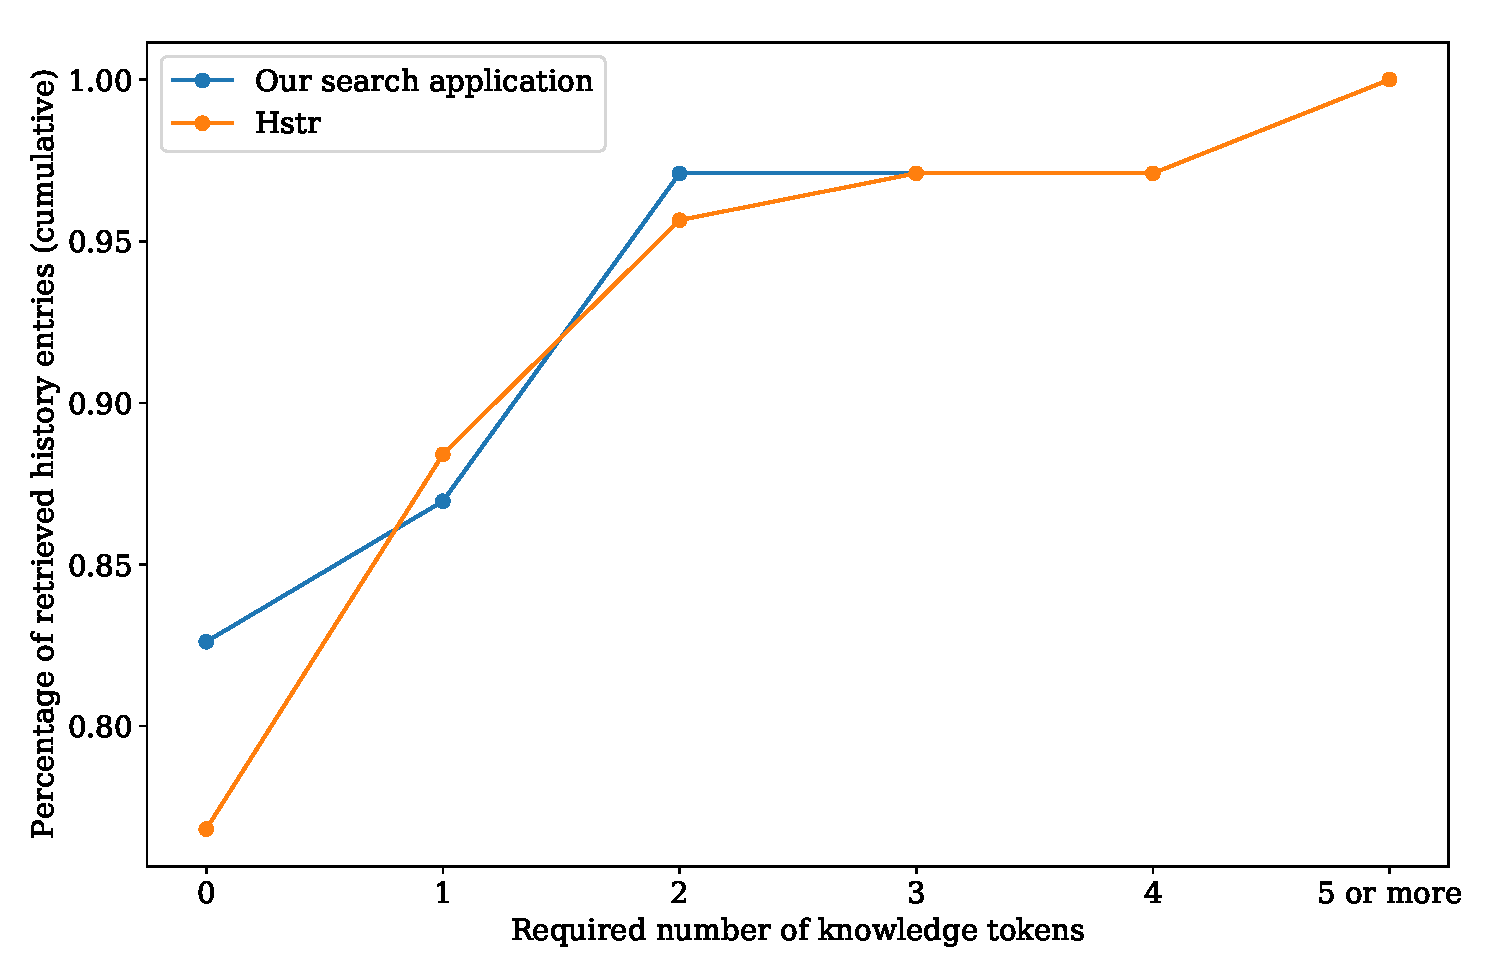
\includegraphics[width=0.97\linewidth]{figures/testing/testing-metrics-cmds-resh.pdf}}
\caption{Cumulative percentage of retrieved history entries as a function of required knowledge (Invocations of our search app.)}
\label{eval-metrics-plot-cmds-resh}
\end{figure}


\begin{figure}[h!]
\centering
\tmpframe{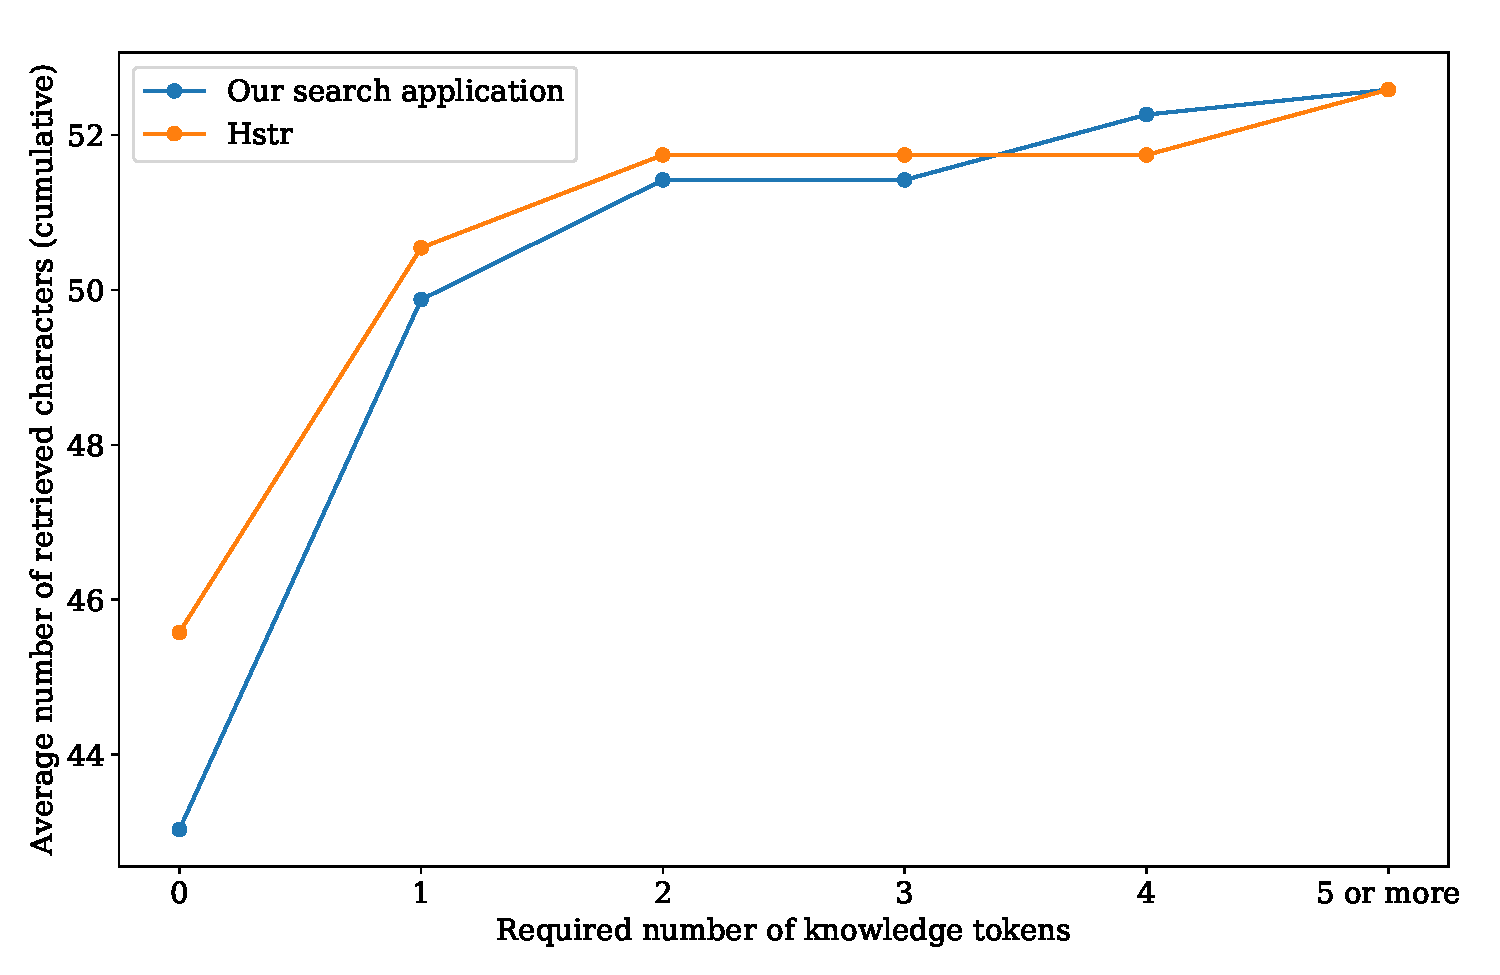
\includegraphics[width=0.97\linewidth]{figures/testing/testing-metrics-chars-hstr.pdf}}
\caption{Cumulative retrieved characters as a function of required knowledge (Invocations of Hstr)}
\label{eval-metrics-plot-chars-hstr}
\end{figure}

\begin{figure}[h!]
\centering
\tmpframe{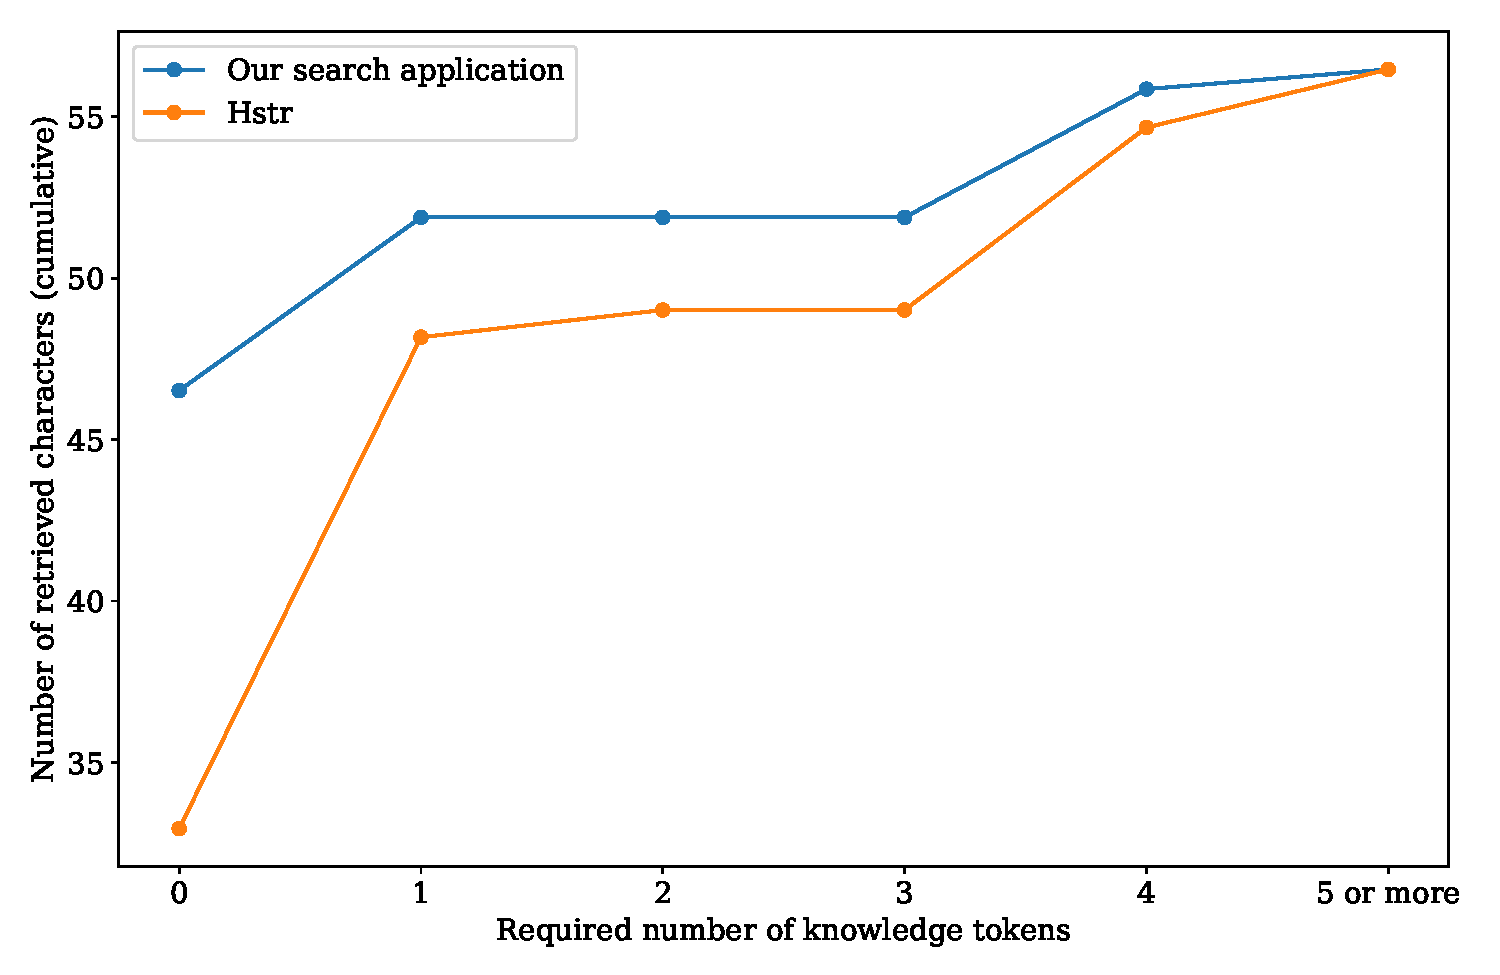
\includegraphics[width=0.97\linewidth]{figures/testing/testing-metrics-chars-resh.pdf}}
\caption{Cumulative retrieved characters as a function of required knowledge (Invocations of our search app.)}
\label{eval-metrics-plot-chars-resh}
\end{figure}

\redtext{TODO: increase the size of the images if you shrink the captions}

\clearpage
\section{User feedback}

In this section, we describe how we released the project to the public, what improvements we made based on interviewing our users, and what feedback we get from users,

We released the first prototype of the search application about five months ago. We are engaging with the community and incrementally updating and improving the project. 

\subsection{User adoption}

Since the release of the first prototype of the search application four months ago the project was downloaded and installed over 600 times. 

The project also received over 250 stars on GitHub which is a bookmarking and endorsement feature on the GitHub website.\cite{github-stars}

% https://keep.google.com/u/0/#NOTE/1pMiUTB0AU_JLmuiPByH7lHyzJR8_brmRqsiOeXRFez5t6wb0OUFtlinZ4oVNGpS9wRl_


\subsection{Feedback from the users}

Here, we describe what improvements we made to the project and what feedback we got from our users. We only mention a few examples of changes and feedback.

\paragraph{Non-contextual mode}

Some of the users were asking for a way to turn off the contextual search because it can occasionally get in their way. For example, logging into remote servers with \verb|ssh| can be done regardless of current directory. When searching for past \verb|ssh| commands the contextual search might do more harm than good.

Based on this we have added the ability to switch between contextual and non-contextual mode with \verb|CTRL-R|. This way the user can always choose the appropriate tool for the specific situation.

\redtext{ADD screenshot}

\paragraph{More ergonomic arrow key bindings}

One of our users was complaining that he is used to repeatedly pressing \verb|CTRL-R| to navigate to between the search results. He was previously using the standard reverse search.

By interviewing the user we discovered that he needs more ergonomic key bindings for arrow keys because they are quite far away from the home row. We have added alternative emacs-inspired bindings for arrow keys; Pressing \verb|CTRL-N| selects the next result on the page and \verb|CTRL-P| selects the previous one.   


\paragraph{Special handling for exit status}

We got some feedback regarding using exit status as part of contextual search. When users kill the running command using \verb|CTRL-C| it exits with the status of 130.
We anticipated that this would happen but it is more common than we expected.
We could add special handling for exit statuses that have special meaning.

\redtext{SKIP ?}
\begin{itemize}
    \item Better help / onboarding
    \item Directory jumping - history vs. specialised tools
\end{itemize}

\subsection{User testimonies}

Now, we sum up what people say about the project. 

In our sizeable user base we have people who have switched from Hstr to our history system. Multiple people have said that our search application have fully replaced Hstr in their workflows. Based on this we conclude that we provide a reasonable alternative to Hstr.

We shared the project online on multiple occasions and the feedback we received from people is overwhelmingly positive.\cite{resh-feedback}

\section{Additional workflows}

In this section, we describe additional workflows that are possible to complete using our search application. 

\subsection{Quickly retrieve history from other sessions}

Since standard history is handled individually in each session users cannot access history from other simultaneously running sessions. 

Our search applications uses history from all running sessions immediately. This means that user can quickly access history from another open terminals. 

Specifically, pressing \verb|CTRL-R| twice launches the search application and switches to non-contextual mode. This way the user can see all recent history entries from all sessions.

\subsection{Find similar history entries}

When the search application is launched, the contents of the command line are used as the initial query. For example, the user can use \verb|ARROW_UP| to retrieve the previous history entry and then press \verb|CTRL-R|. 

Using a full command line entry as a query fills the page with similar history entries. This is possible because of properties of our scoring function; It returns reasonable results even when there are words in the query that do not match anything. 

\subsection{Write new command line entries based on history}

Sometimes we want to write a new command line entry but we do not quite remember all of its parts. To make the writing easier it would be useful to see other similar history entries while writing.

As we already mentioned, when launching the search application the contents of the command line are used as a query. Conversely, the user can press \verb|CTRL-G| to abort the search and the contents of the query are pasted back onto the command line.
Combination of these two actions makes it possible to transfer back and forth between the command line and the search application. 

All this can be used to write new command line entries while

We can launch the search application and start writing the command line into the query field. The search application continuously shows us similar history entries we can use as an inspiration. When we are done with typing the command line entry, we use \verb|CTRL-G| to get back to the command line. Then, we can execute the command line entry.


